\documentclass{article}

% Language setting
% Replace `english' with e.g. `spanish' to change the document language
\usepackage[english]{babel}

% Set page size and margins
% Replace `letterpaper' with `a4paper' for UK/EU standard size
\usepackage[letterpaper,top=2cm,bottom=2cm,left=3cm,right=3cm,marginparwidth=1.75cm]{geometry}

% Useful packages
\usepackage{amsmath}
\usepackage{authblk}
\usepackage{lmodern}
\usepackage{graphicx}
%\usepackage{todonotes}
\usepackage[section]{placeins}   % helps to keeps figures at the same page or within the /FloatBarrier
%\usepackage{caption}    % lets you define the fontsize of figure captions
\usepackage{subcaption}
\usepackage[colorlinks=true, allcolors=blue]{hyperref}

%added by LK
\usepackage{textgreek}
\usepackage{ltablex} %have centerised tables

\renewcommand\Authfont{\fontsize{9}{10}\selectfont}
\renewcommand\Affilfont{\fontsize{8}{9}\itshape}

\title{Implementation of an On-Board Terrain Classifier based on Proprioceptive Sensor Data for a Planetary Rover}
\author[1]{Raul Dominguez}
\author[2]{Lennart Kuhr}
\author[1]{Jonathan Babel}
\author[1]{Florian Cordes}
\author[3]{Giulio Reina}
\author[1,4]{Frank Kirchner}
\affil[1]{DFKI Robotics Innovation Center Bremen Robert-Hooke-Str. 1, 28359 Bremen, Germany, \newline E-mail: name.surname@dfki.de}
\affil[2]{Institute of Space Systems, TU Braunschweig, Herman-Blenck-Straße 23, 38108 Braunschweig, Germany, \newline E-mail: l.kuhr@tu-braunschweig.de}
\affil[3]{Department of Mechanics, Mathematics and Management, Polytechnic of Bari, Via Orabona 4, 70125, Bari, Italy, E-mail: giulio.reina@poliba.it}
\affil[4]{Robotics Research Group, University of Bremen, Germany}

\begin{document}

\date{}
\maketitle
\captionsetup[figure]{font=footnotesize}
\captionsetup[table]{font=footnotesize}

\begin{abstract}
The implementation of a Support Vector Machine-Based terrain classifier for the hybrid locomotion rover SherpaTT is presented. 
The first phase of classification consists of deriving the physical characteristics of the traversed terrain statistically from proprioceptive data (i.e. engineered features).
The features are then used by the classifier to distinguish between three different surface types: \emph{sand}, \emph{compact sand} and \emph{concrete}. 
Based on previous offline studies \cite{Dimastrogiovanni2020} the terrain classifier has been integrated into the control architecture of the rover, as well as deployed and tested in analog environment. 
The software runs completely on the onboard computer (OBC) of SherpaTT, embedded within the Robotics Construction Toolkit (Rock)\footnote{Rock: The Robot Construction Kit (\url{http://rock-robotics.org})} framework.
Insights on the implementation and the software architecture surrounding the classifier are provided. 
Performance metrics demonstrate that the terrain classifier can run on the OBC alongside with the rest of the control architecture, achieving an overall high accuracy in terrain classification.
\end{abstract}

%\todo[inline]{We have to limit the paper to 9 Pages}

\section{Introduction}

% Introduction main motivation and main idea of the paper explain in detail the implementation of a SMV-based proprioceptive terrain classifier
Planetary explorations missions are so far dominated by wheeled rover designs like Curiosity
or Perseverance \cite{moeller2021, welch2013}. Although wheeled locomotion is most energy-efficient
over flat terrain, it compromises drawbacks when exposed to demanding unstructured
terrain. Especially in unstructured environments with steep, sandy slopes and boulders
patches, wheeled systems reach their limitations \cite{kolvenbach2021}. In the past, several high slip and
excessive sinkage events have been encountered with exploration rovers, which have severely
disrupted mission timelines \cite{gonzalez2018}. It took five weeks to free the Opportunity
rover from sand in 2006 \cite{young2006} and rover trajectories need to be frequently adjusted to avoid
challenging terrain \cite{arvidson2017}. The potentially worst situation occurred in 2009, when the
Spirit rover got stuck in sand and was unable to recover, ultimately ending the mission
\cite{webster2009}. 
Terrain awareness, the correct modelling of transited surfaces and its classification is a key factor for reliable autonomous navigation. 
Surface modelling can be used for navigation in order to avoid operation problems like the ones previously described. 
Moreover, terrain awareness may enhance navigation capabilities, if drive settings are adapted in accordance to the 
terrain properties.

In this publication we introduce a software component capable of classifying three different terrain types based on the proprioceptive sensor data of SherpaTT. 
The component uses a Support Vector Machine (SVM) algorithm \cite{vapnik1992,cristianini2000} in its core. It is integrated into the software control architecture of the mobile exploration robot SherpaTT embedded into the Robotics Construction Toolkit (Rock) framework, such that it can be executed sufficiently fast during navigation. The terrain classifier uses force torque sensors, joint data and body acceleration estimates to classify the surface into one of three terrain types: \emph{sand, compact sand} and \emph{concrete}.
The three types represent distinct classes of surfaces characterized by its deformability and friction properties. In order to achieve a better classification performance as well as a more in-depth characterization of the surface patches, a feature calculation process is performed previous to the classification. 
%\todo[inline]{RD: Some small state of the art here would be interesting presenting what others have done, not long but at least presenting some similar works}

%Moreover, the classification performance achieved onboard SherpaTT was identified during tests on terrain that represent at least one of the three terrain type classes.

\section{Background}

% NOTE: This text is just a short introduction of what is coming in the next 3 subsections, if it is too repetitive we can remove it.

\subsection{SherpaTT}

SherpaTT is a hybrid wheeled-leg rover with an actively articulated suspension system. Its locomotion control system provides the basis for advanced locomotive capabilities with the ability to adapt to different terrain types \cite{cordes2018}. The rover is designed for operation in unstructured environments. It features terrain adaption based on force torque sensors inputs, trajectory control and path planning as well as environment reconstruction through data fusion of extereoceptive and proprioceptive data. The placement of the sensors, that provide propriocepitve input data to the terrain classifier on SherpaTT, is shown in Figure~\ref{fig:SensorInputs}. The purpose of the high mobility platform is to access scientifically interesting areas on planetary bodies in a safe, fast and autonomous way. Besides the enhanced locomotion system, SherpaTT benefits of its’ advanced motion control system (MCS). The MCS guarantees controlled articulation of the complex kinematic suspension system at any time. It is implemented as a middle-layer between high-level processes and the low-level hardware layer, shown in Figure ~\ref{fig:MCS}. The layer architecture of SherpaTT can be described as such \cite{cordes2018}:

\begin{figure}[!htbp]
   \subcaptionbox{
       \label{fig:SensorInputs}Sensor and joint inputs to the Terrain Classifier
       }
       {
           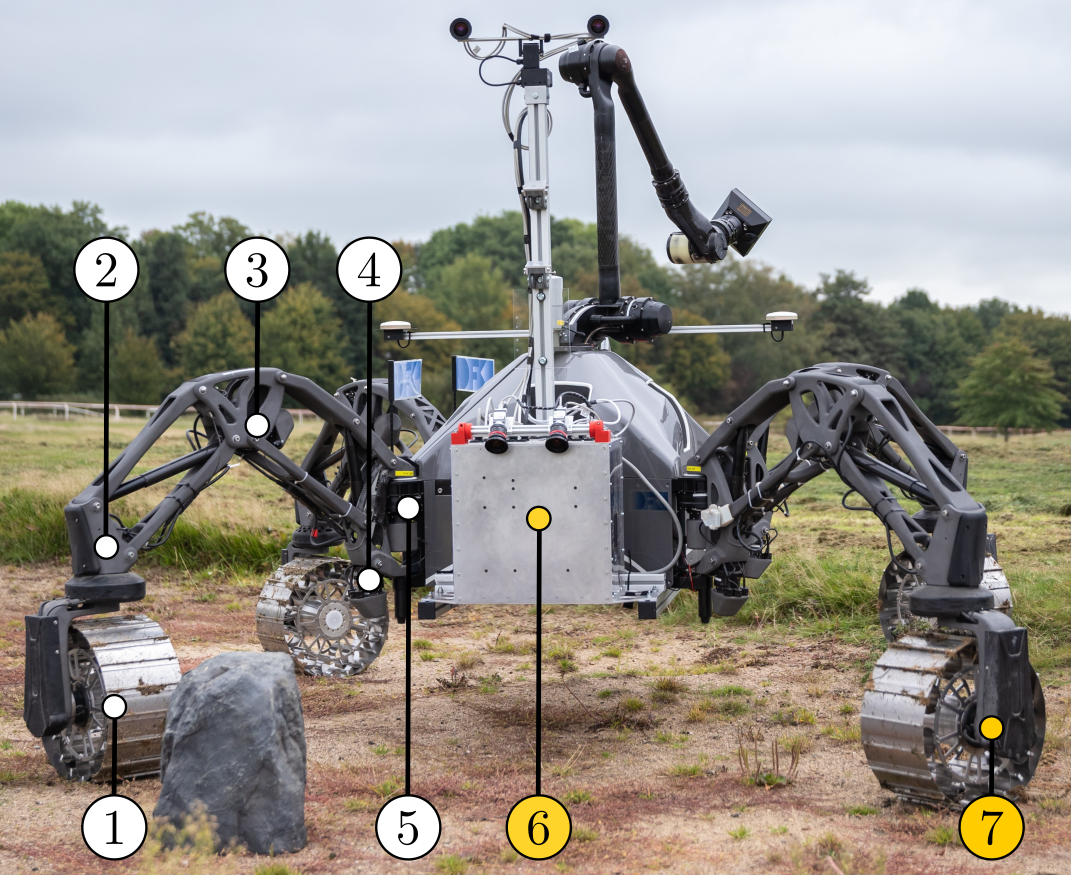
\includegraphics[width=0.45\textwidth]{../figures/terrain_classifier_sensor_inputs.png}
       }
   \subcaptionbox{
       \label{fig:MCS}Motion Control System of SherpaTT \cite{cordes_phd_2018}
       }
       {
           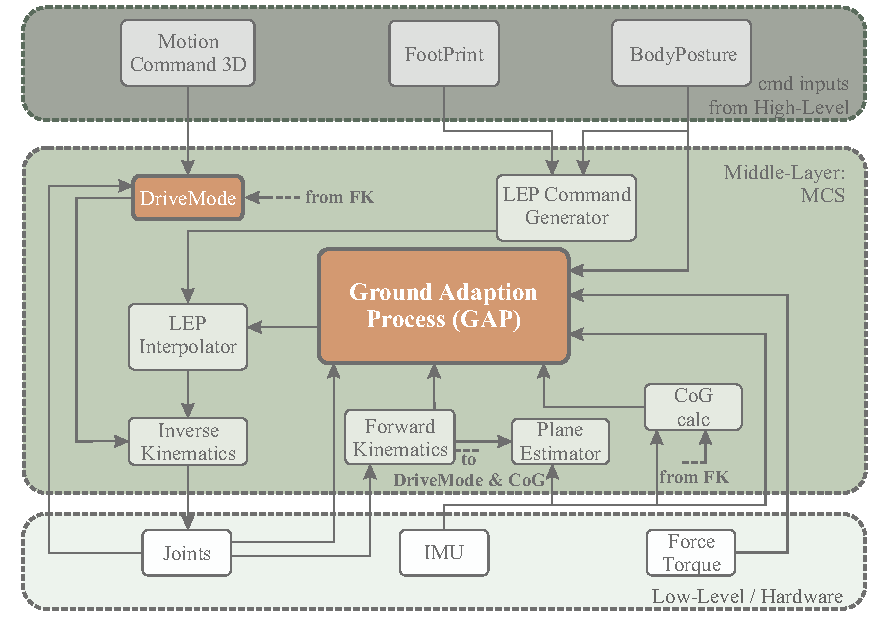
\includegraphics[width=0.5\textwidth]{../figures/MCS-Structure.pdf}
       }
   \caption{\label{fig:Loco}(a) Input features for the terrain classifier originate from the following actuators (1)-(5) and sensors (6)-(7) on SherpaTT: (1) wheel drive, (2) wheel steering, (3) linear knee, (4) linear shoulder, (5) pan shoulder, (6) IMU, (7) Force-Torque. (b) Simplified layout of the Motion Control System of SherpaTT. Source: F. Cordes.}
\end{figure}

\begin{itemize}
    \item \textbf{High-Level:} Is the autonomy level of the robot’s control system. Resembles for example navigation, mapping or path planning software. Related behaviors are independent of the physical states of the robot.
    \item \textbf{Middle-Layer:} Resembles an abstraction of the physical robot. Handles command inputs from the operator or high-level processes and calculates according joint movements. It reacts to sensor inputs and thereby assures system stability for example by monitoring the position of the Center of Gravity (CoG) to avoid tip-over.
    \item \textbf{Low-Level:} Is close to the physical hardware. This comprises sensors and local joint controllers for example PID controllers for position or velocity control of an individual joint. Besides providing commands to the drive actuators, the MCS design aims to mimick passive suspension with controllable properties.
\end{itemize}




\subsection{Development Tools}

The software enabling the control and perception mechanisms of SherpaTT exchanges data and information through the Robotics Construction Toolkit (Rock) framework. 
The framework not only provides wrapping mechanisms for the libraries and its communications, but also the possibility to enforce realtime execution of the control loops when using a realtime supporting Linux kernel. 
Rock offers a set of useful tools for the development, testing and evaluation of the software libraries (e.g. runtime data exchange statistics and visualization). 
In particular, tools for data logging, replaying and memory-signature based data selection from data streams have been employed in this implementation. 

% Challenges
Data selection at runtime is on of the key features addressed by the middleware. 
The problem consists in generating matrices of synchronous sample values for classification online from data streams with multiple frequencies.
Each data stream relevant for the classification contains in addition to the relevant data, data which has to be filtered out (e.g. timestamps) since it is useless for the classification.
The library \emph{type to vector}\footnote{Type to vector: \url{https://github.com/rock-data-processing/data_processing-orogen-type_to_vector}} is used to select the fields of the datatypes in the samples of the data stream. 
It uses the type memory descriptions of the samples which contain relevant data to select from the incoming streams only the relevant attributes and stack them into the input matrix. 

The synchronicity of the data that is inputed to the classifier is achieved using the timestamps with which the sensor data is marked at acquisition time.
Data streams can have different update rates, but the input matrices need data from multiple sources at the same rate, therefore a strategy is needed to drop or interpolate data. 

The Rock logging mechanism, is used to store in hard drive the sensor and fused data streams while traversing for later use offline (i.e. data collection). 
Two further tools are employed to process the logged data offline: rock-replay for testing the runtime functionality on the development environment and \emph{pocolog to msgpack}\footnote{Pocolog to Msgpack: \url{https://github.com/rock-core/tools-pocolog2msgpack}} to select and prepare the data, so that it can be employed for training and testing the classifier.
\emph{pocolog to msgpack} converts data from its rock binary representation to the almost universal \emph{msgpack} format.
Moreover, \emph{pocolog to msgpack} allows for the conversion of logged data into python data frames, the widely used python data science and machine learning format. 
Finally, the runtime inspection tools of Rock were utilized to monitor the processing time of the classifier, the connections between separate software components and to visualize the coherence of all input data streams. 


\subsection{Terrain Classifier}
% Background and approach

In order to classify three terrain types using proprioceptive sensor data, the supervised machine learning algorithm Support Vector Machine (SVM) is utilized. 
Applying such algorithm requires the training of a SVM classification model that is later used to classify n-dimensional datapoints.
The model's dimensions are called features and they correspond to the inputs that are used for guessing the class. 
SVM separates the data among classes, during training the boundaries among the different classes are adapted. 
The more separation that is achieved between the classes, the clearer the later classification of datapoints is expected. 
In order to the achieve maximum separation between the data classes, the optimal features, computed from the sensor data, need to be identified. 
In other words, a feature selection process allows to identify the most critical set of input data to the classifier. 
%features differs in performance  
%feature selection

\paragraph*{Model Training}
%\subsubsection{Model Training}
Generally, SVM aims to separate data of multiple classes. 
In geometrical terms it divides the data with a n-dimensional hyperplane, the so called decision boundary. 
The hyperplane parameters, or so called weights, are iteratively optimized to allow the largest distance between the hyperplane and the nearest datapoints which eventually are the support vectors.  
By changing the dot-product calculation, which is referred to as the kernel trick, within the underlying geometrical condition various correlations of the data's dimensions can be recognized. 
Example correlation can be obtained through polynomial or Gaussian radial based function.
However, the most simple is linear correlation.
The generated set of weights is referred to as \emph{classification model} and the generation process as such is referred to as \emph{training}.%\cite{kuhr2021}
%OvA multiclass strategy



%\subsubsection{Model Testing}
\paragraph*{Model Testing}
Before deploying the model, its' classification performance can be measured using labeled data.
This testing process obtains the performance measures are tipically visualized within \emph{confusion matrices}. 
A description of the three class confusion matrix which is used to present the results in this work is depicted in Figure~\ref{fig:CMdescrpit}
The three evaluated aspects or performance measures are \emph{precision}, \emph{recall} and \emph{accuracy}.
The process done by the classifier of processing a sample and providing a classification label is also referred as prediction.
\begin{itemize}
\item \textbf{Accuracy} measures the overall percentage of correctly classified samples: $\frac{T\textsubscript{overall}}{(T+F)\textsubscript{overall}}$ 
\item \textbf{Recall} measures for each set of samples of each class the percentage that was correctly classified: $\frac{T\textsubscript{class}}{(T+F)\textsubscript{actual class}}$%: Out of all samples that belong to an actual class does the classifier classify the correct class 
\item \textbf{Precision} measures for each set of predictions per class the percentage of predictions that were correct: $\frac{T\textsubscript{class}}{(T+F)\textsubscript{predicted class}}$%: Out of all classifications that the classifier assigns to one class does the classifier classify correctly
\end{itemize}
Where $T$ stands for True (correct) and $F$ for False (wrong).

\begin{figure}[!htbp]
    \centering
    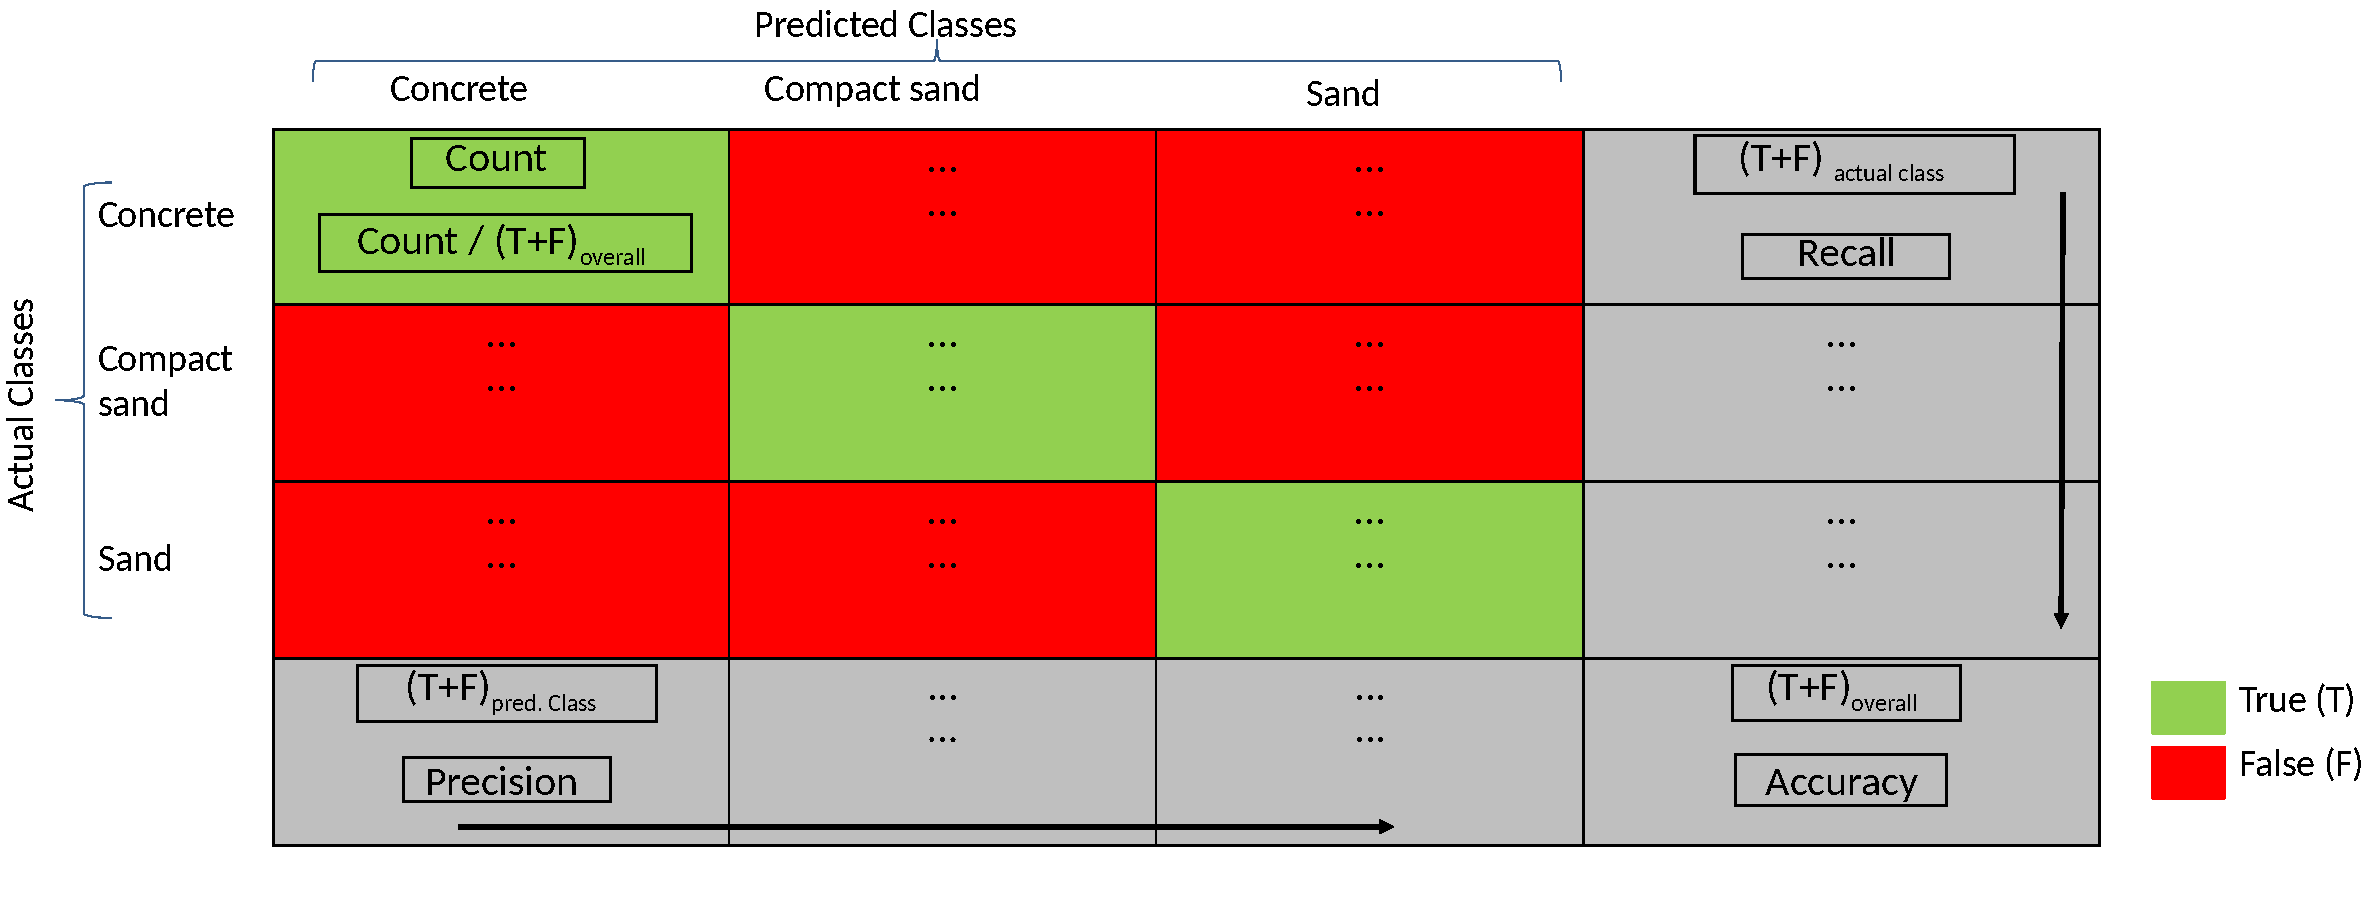
\includegraphics[width=0.7\textwidth]{../figures/CM_Description.pdf}
    \caption{\label{fig:CMdescrpit} Confusion matrix used to visualize the performance measures, \emph{Precision}, \emph{Recall} and \emph{Accuracy}, of the classifier.\cite{kuhr2021}}
\end{figure}


%\subsubsection{Feature Selection}
\paragraph*{Feature Selection}
For computational reasons as well as for simplicity, it is desired to reduce the dimensionality by selecting the most critical features for the  classification task.
Within the selection process, a large set of statistical moments of the features are considered. 
The features can represent direct sensor parameter as well as physical parameters such as the mechanical and electrical power, friction coefficients and the wheel speed deviation of each wheel in relation to the others. 
The proprioceptive sensor data used to calculate the features are listed in Table~\ref{table:features1} which is based on \cite{Dimastrogiovanni2020}.
The input data is received from the Motion Control System (MCS), Joint Deployment (JD), Sensors Deployment (SD). 
All forces and torques are represented within the Body Coordinate System (BCS).

\begin{table}[!htbp]
   \centering
    \begin{tabularx}{\columnwidth}{XXX}
    \textbf{Symbol}& \textbf{Feature} & \textbf{Datastream}  \\
    \hline
      $F\textsubscript{x}$ & Longitudinal Force	 &  MCS\\
      $F\textsubscript{z}$& Vertical Force	 &MCS \\ 
      $T\textsubscript{y}$& Drive Torque around y-axis	   &MCS\\ 
      $I $& Motor Current	  & JD\\ 
      $V$ & Voltage 	   &JD\\ 
      $d\textsubscript{pwm}$&  Dutycycle	   &JD\\ 
      $w$& Angular Wheel Velocity 	 &JD \\
      $a\textsubscript{x}$& Acceleration X	  &SD\\ 
      $a\textsubscript{z}$&  Acceleration Z	   &SD\\ 
    \end{tabularx}
    \caption{Proprioceptive inputs and supplying datastream}
    \label{table:features1}
\end{table}

Using the inputs in Table~\ref{table:features1}, the physical statistical features listed in Table~\ref{table:features2} are calculated for each patch of terrain to be classified.
The statistical moments mean, variance, skewness and kurtosis were evaluated initially. 
A selection of the most useful features for the classification, to reduce dimensionality was done using the WB index and the Pearson Coefficient.
Both the equations for the calculation of the physical features as well as the details on the selection process of the most critical features are detailed in \cite{Dimastrogiovanni2020}.

\begin{table}[!htb]
   \centering
    \begin{tabularx}{\columnwidth}{XXX}
    \textbf{Statistical} & \textbf{Feature}  & \textbf{Symbol} \\
    \hline
     M,SD	&  Longitudinal Force	 & F\textsubscript{x} \\ 
     M,SD	&  Drive Torque	around y-axis  & T\textsubscript{y} \\ 
     M,SD	&  Drive Current	 & I \\  
     M,SD	&  Acceleration X	 &  a\textsubscript{x}\\ 
     M,SD	&  Acceleration Z	 & a\textsubscript{z} \\ 
     M,SD	&  Mechanical Power	 & P\textsubscript{m} \\ 
     M,SD	&  Electrical Power	 & P\textsubscript{e} \\ 
     M,SD	&  Friction Coefficient 1	 & \textmu \textsubscript{1} \\ 
     M,SD	&  Friction Coefficient 2 & \textmu \textsubscript{2}\\ 
     M,SD	&  Friction Coefficient 3	 & \textmu \textsubscript{3}\\ 
     M	    &  Angular Wheel Velocity	     &  w      \\ 
     SD    	&  Speed Deviation	 & $\Delta$w\\ 
    \end{tabularx}	
    \caption{Optimal feature set for the classification of terrain types by SherpaTT. The set includes the statistical calculation of mean (M) and standard deviation (SD) per terrain patch.\label{table:features2}}
\end{table}

%\subsubsection{Linear Discriminant Analysis}
%copy paste from thesis
%\paragraph*{Linear Discriminant Analysis}
%Besides speeding up the training and reducing the required amount of data during runtime, the reduction of feature dimensionality can help for data visualization. 
%Linear Discriminant Analysis (LDA) reduces the number of dimensions down to the three or two more representative. 
%This makes it possible to plot a high-dimensional data set on a graph and through this visually gain information about patterns. 
%
%To achieve this, LDA identifies the axis that accounts for the largest amount of variance of different class's data. 
%It thereby represents a similar method as the Principle Component Analysis (PCA) with the difference that LDA recognizes the class labels when identifying the variance. 
%As a next step, LDA identifies the axis that lays orthogonal to the first one. 
%Therefore, the second axis accounts for the largest amount of remaining variance. 
%The maximum number of orthogonals, linear discriminants, depends on the number of dimensions within the data set.\cite{kuhr2021}
%

\section{Implementation}

The classifier control loop has a target frequency of 100 $Hzs$, matching the highest input frequency (joint status). 
To address the issue of other streams having lower frequency, the simple solution of using the same data as input for several entries in the classifier input matrices was taken. 
The classification is performed on matrices composed from information generated from 100 samples. 
Thus a classification is generated every second.
In other words, every 100 samples, a matrix input for the classifier is completed and a new classification is done, this happens every 1 $s$.
Since the speed of the rover was 0.1 $m/s$, the resolution of the categorized patches of terrain is 10 $cm$ long.  


The classification results need to be available at a fast enough pace to allow other onboard components take advantage of the results (e.g. to improve navigation) and to ensure that the classification results correspond to the currently traversed surface. 
Likewise, the loss of data samples due to full queues on the input of the processing components must be avoided. 

The diagram in Figure~\ref{fig:overview} presents the implementation approach of the terrain classifier in Rock. 
The first step which needs to be done efficiently is the extraction from the data sample of the relevant fields of data which is done using the \emph{type to vector} Rock tool.
At each execution of the \emph{updateHook} (every 0.01) new data is stacked in the input matrix.
Every 100 \emph{updateHooks} an input matrix is finished and the component triggers the computation of the physical and statisticall features and finally the classification, also named prediction.
The output of the classification as well as the of the feature computation are delivered to the calling component which retrives the values through its output ports. 

\begin{figure}[!htbp]
    \centering
    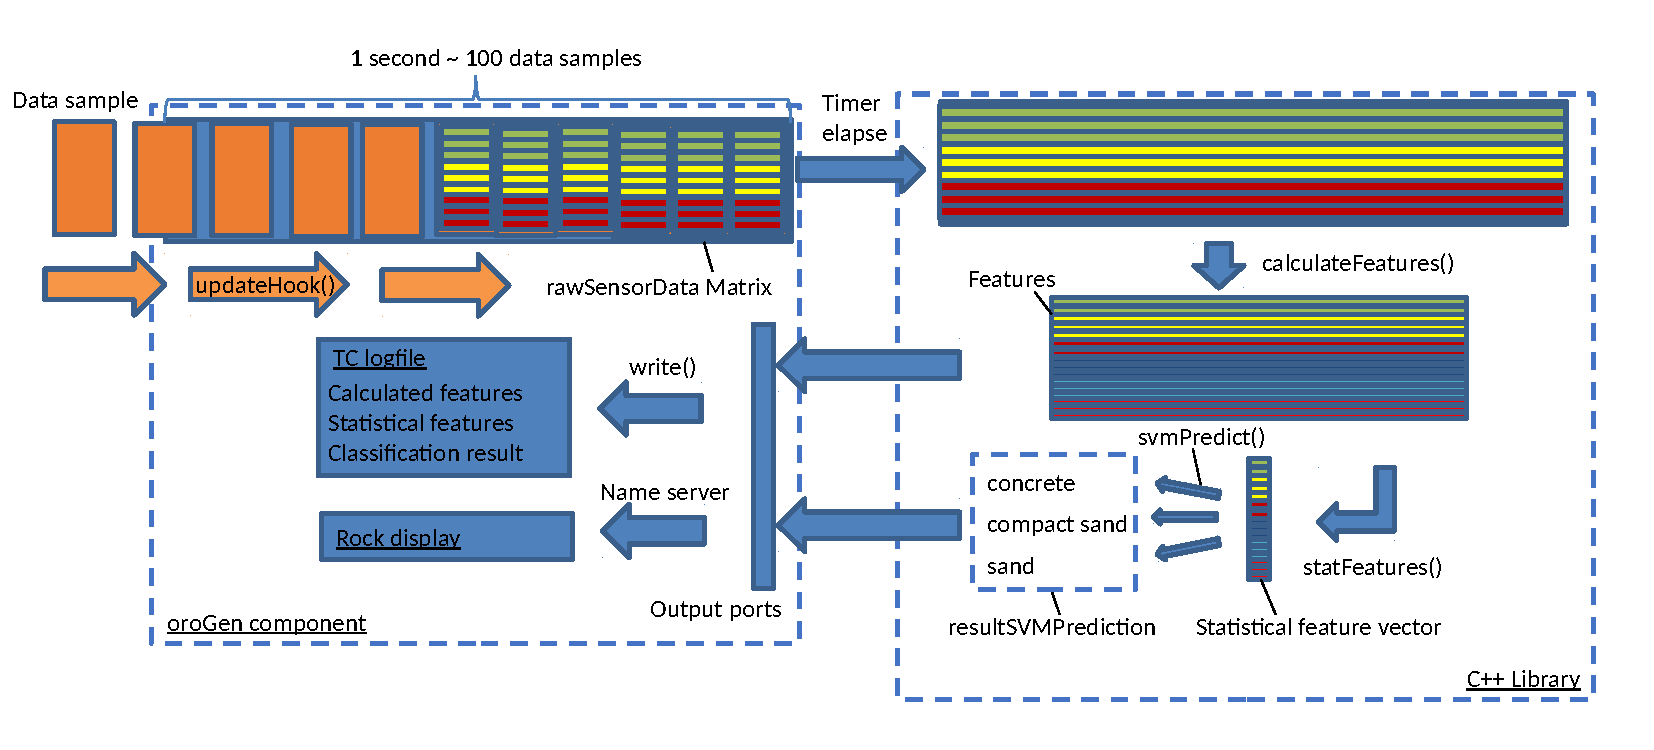
\includegraphics[width=0.9\textwidth]{../figures/OverviewTC2.pdf}
    \caption{\label{fig:overview}Overview of the terrain classifier library and Rock integration.}
\end{figure}

\subsection{Training Data}

An essential aspect needed to achieve a good classification performance is to have a consistent and large data collection available for training and testing. 
The data collection available for this implementation consists of a dataset composed of traverses that were acquired by remote commanding the rover over the 3 examined terrain types: \emph{loose sand}, \emph{compact sand} and \emph{concrete}. 
One traverse in the dataset corresponds to the forward and backward driving of 10 $m$. 
The following conditions were the same during all traverses: (1) Fixed wheel configuration, (2) Surfaces without inclination, (3) Traverse speed 0.1 $m/s$, (4) Straight traverses and (5) Electric power generator is running, which causes vibrations.
Figure~\ref{fig:TestLocs} shows images of the rover traversing the different terrains during the data collection.


\begin{figure}[!htb]
   \centering
    \subcaptionbox
        {Loose Sand}
        {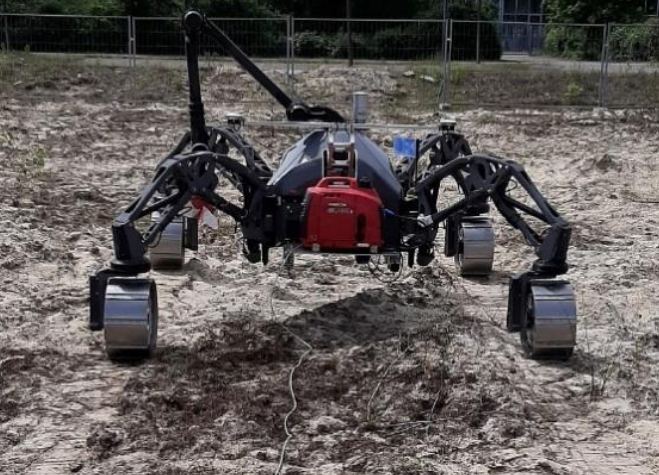
\includegraphics[width=0.32\textwidth]{../figures/unprepsand.png}}
    \subcaptionbox
        {Compact Sand}
        {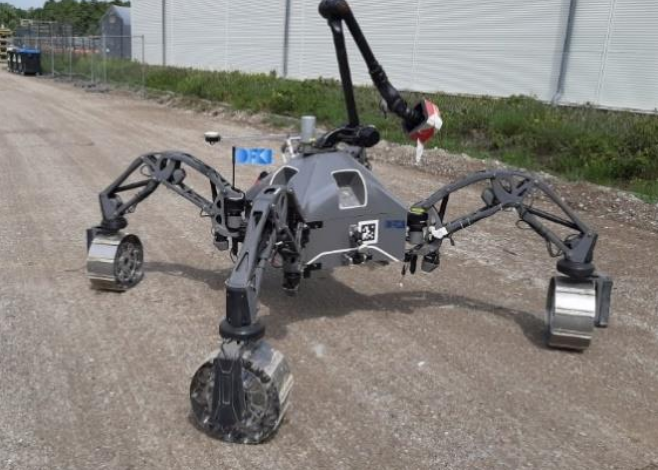
\includegraphics[width=0.32\textwidth]{../figures/compact.png}}
    \subcaptionbox
        {Concrete}
        {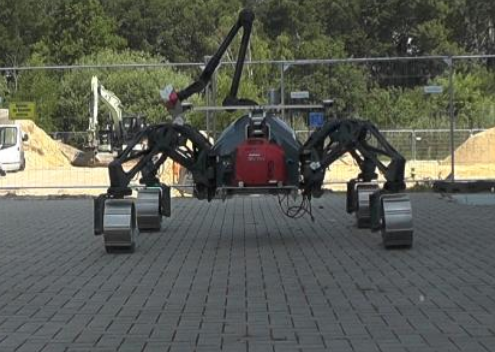
\includegraphics[width=0.32\textwidth]{../figures/concrete_v2.png}}
    \caption{The test locations where the data sets were acquired.}
    \label{fig:TestLocs}
\end{figure}



In terms of quantity, the data collection consists of 2200 training samples for each of the 76 features. 
Regarding data balance, the data gathered from the terrain type loose sand represent 28\% of the total and the concrete and compact sand represent 36\% each. 
When generating a SVM model, the available data collection is divided into training and testing sets. 
For the presented classifier one of the traverses of each terrain is used for testing and all other traverses are used for training. 
This gives a ratio of about 25\%/75\%.

\section{Evaluation}
\subsection{Offline Classification Performance}
%\todo[inline]{RD: TODO for @LK: Provide the results that were collected when testing offline}
%The SVM model training software is implemented to enable the use of a variable constellation of logged datasets. Moreover, it can be used to compare both the offline and online classification performance. 

The components of a Linear Discriminant Analysis (\emph{LDA}) are plotted to visualize the achieved data separation. 
In the LDA two Linear Discriminant components are represented on the axes, these components are formed from a reduction of the original feature set.
Figure~\ref{fig:offline-class}(a) shows the dataset LDA plot and highlights the decision boundary of the trained linear SVM kernel. 
The areas of different terrain types are highlighted by the corresponding colors. 
It is shown that the data of the terrain types can be separated for most of the samples.

The offline evaluation of the SVM classifier reached an accuracy of 93.97\% depicted in the confusion matrix in Figure~\ref{fig:offline-class}(b). 
A small portion of the collected data where SherpaTT was not moving was sliced out. 
Based on the sliced data the classification accuracy could be increased by 2\%.
Except the recall for \emph{compact sand} and the precision for \emph{sand} all performances are above 90\%, with an overall accuracy of 93.97\%.

\begin{figure}[!htb]
    \centering
    \subcaptionbox
        {Linear Discriminant Analysis of the dataset}
        {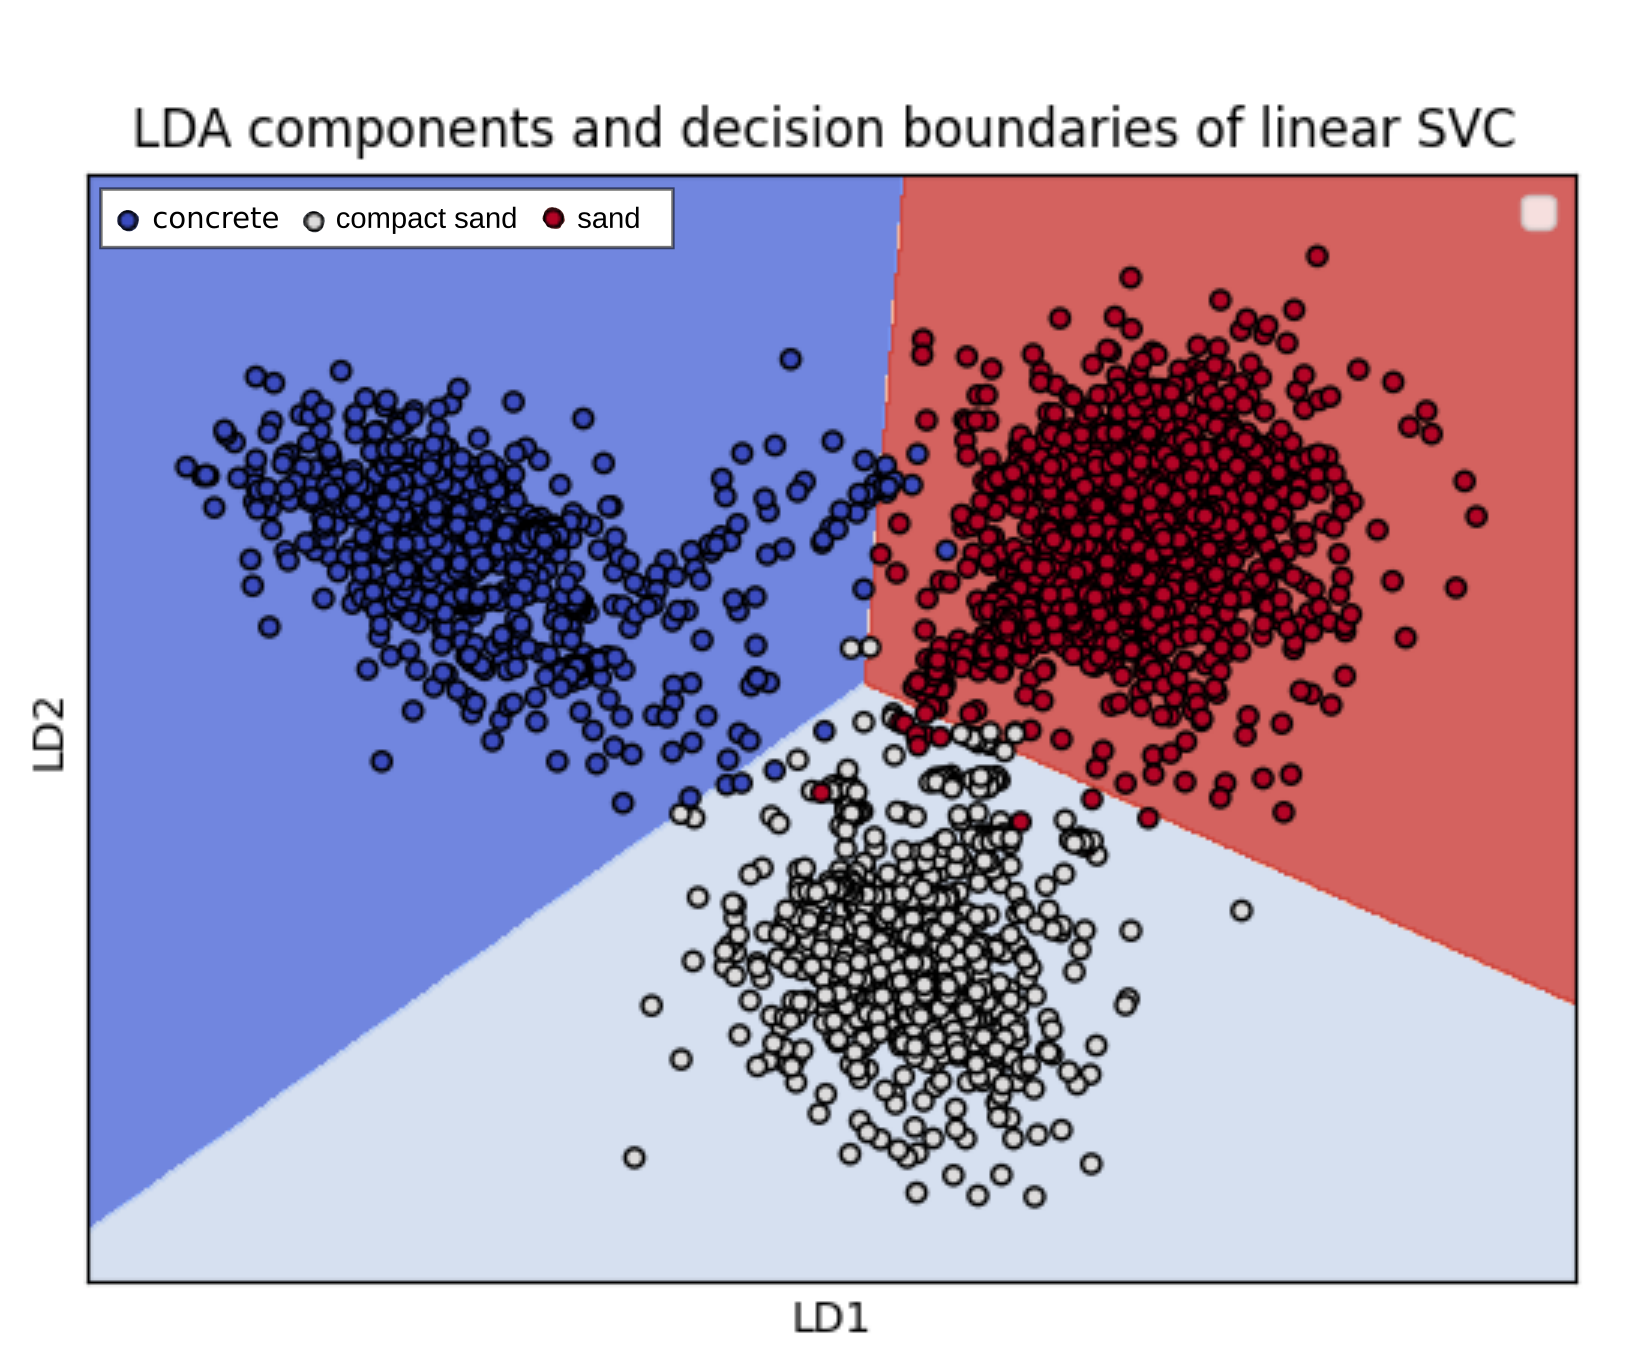
\includegraphics[width=0.48\textwidth]{../figures/boundary_LDA_prevTesting_all_sand_concrete_compactsand.png}}
    \subcaptionbox
        {Confusion Matrix of the terrain classifier}
        {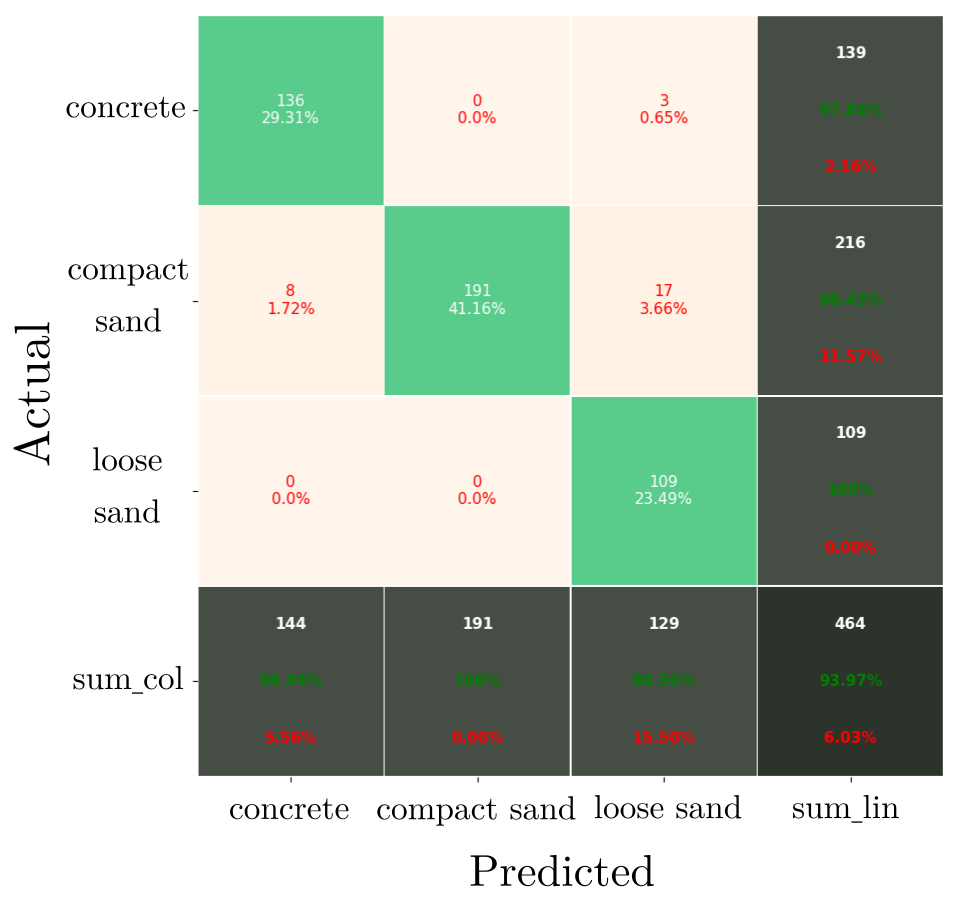
\includegraphics[width=0.48\textwidth]{../figures/confusionmatrix_Train.png}}
    \caption{(a) LDA visualization, the areas of different terrain types as classified by the SVM are highlighted by the corresponding colors. (b) Performance of the SVM model, the overall accuracy yields 93.97\% }
    \label{fig:offline-class}
\end{figure}

\FloatBarrier
% Evaluation

%A complete analysis of performance was not possible, because the traversed terrain during the field tests did not closly match the previously trained terrain classes. Nevertheless, the software shows good classification results, since the type of surface -\emph{wet compact sand}- was close to the two classes mostly identified -\emph{concrete} and \emph{compact sand}.

\subsection{Onboard tests}

Two main tests were performed to validate the onboard calculation of features and classification performance.
The tests consisted of traverses where the component was executing along with the rest of the control and perception sofware components. 

The first of the test was indoors at the DFKI Robotics Innovation Center premises, depicted in Figure~\ref{fig:sh-tests}.
During the test, the classifier ran at the pursued frequency of 100Hz.
Nevertheless, the classification performance of these tests is not considered representative, since the power generator was not active and the hardest surface was not as firm as concrete. 

\begin{figure}[!htb]
    \centering
    \subcaptionbox
        {Loose Sand Tests}
        {
        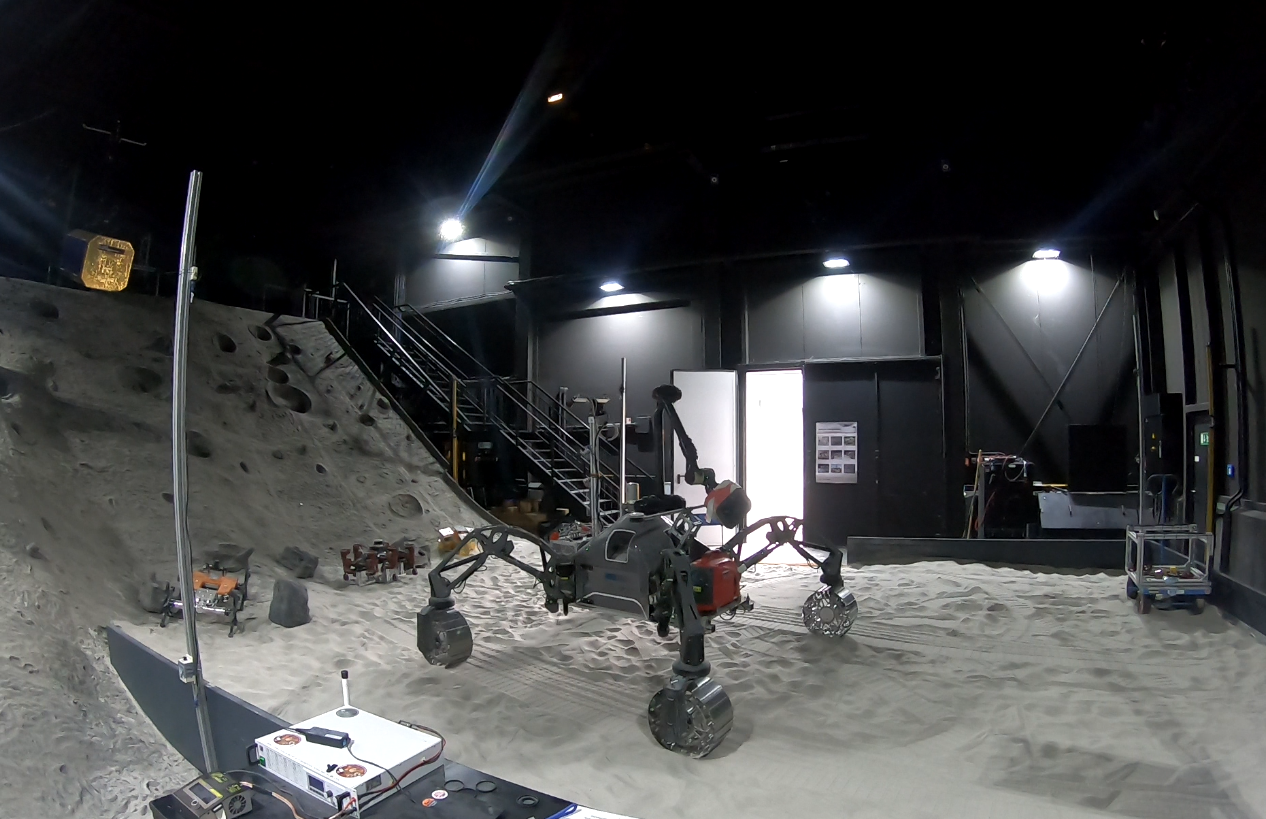
\includegraphics[width=0.4\textwidth]{../figures/spacehall.png}
        }
    \subcaptionbox
        {Concrete Tests}
        {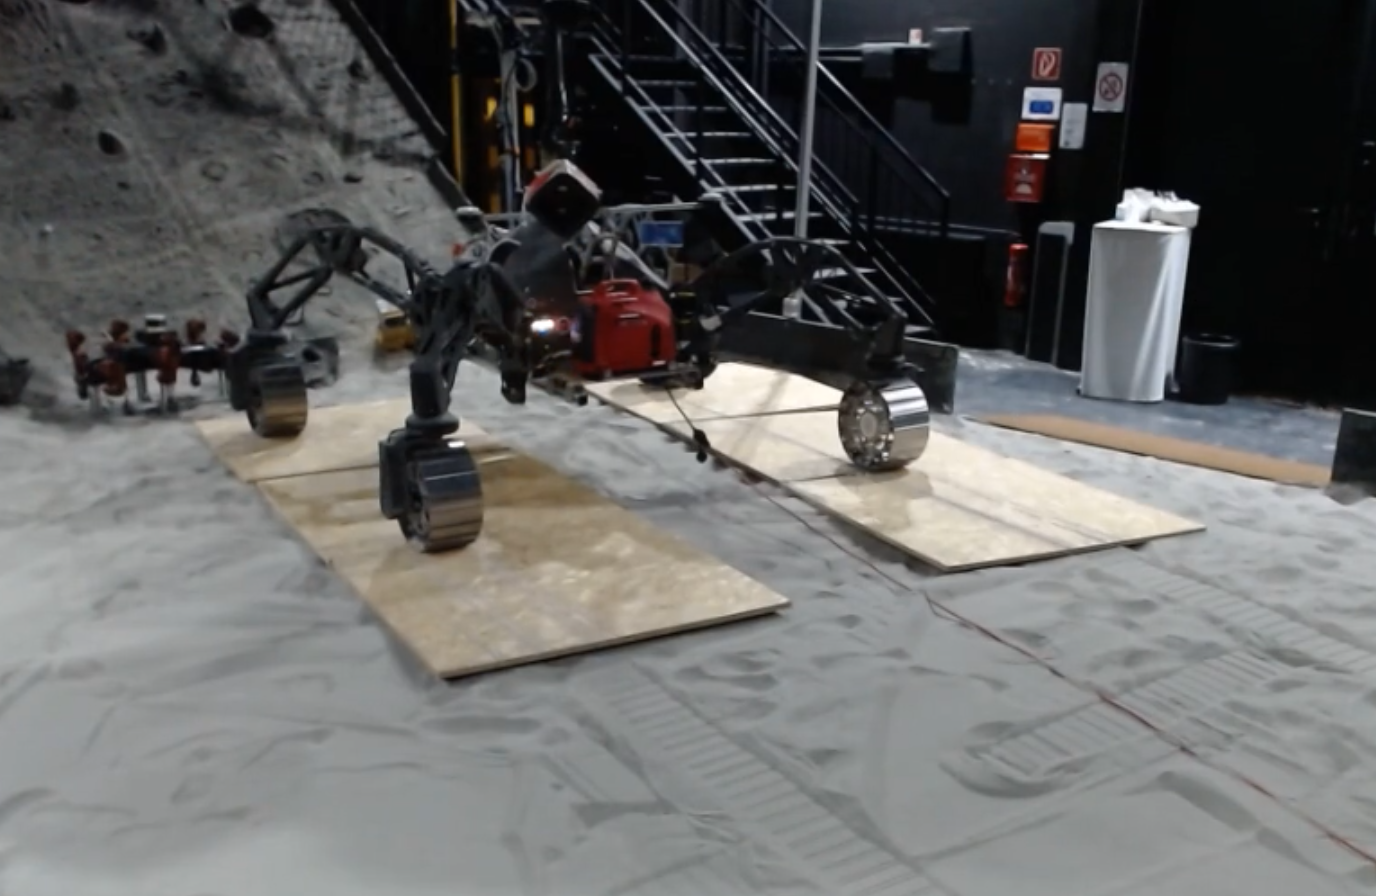
\includegraphics[width=0.4\textwidth]{../figures/spacehallconcrete.png}}
    \caption{Validation of the onboard classifier execution frequencies.}
    \label{fig:sh-tests}
\end{figure}

The second test took place during the final field trials of the ADE project \cite{ocon2021} in a sand mine in Wulsbüttel, Northern Germany.
These tests provided comparable conditions as the ones within the training data set, because the power generator was activated. 
Several traverses of SherpaTT were logged and checked for consistency to validate the feature calculation. 
The classification accuracy reached 87\%. 
A well balanced recall and precision values of the classes were also achieved. 
The underperformance in the field tests are explained by the encountered surface, which did not exactly match any of the previously examined types. 
Due to rainfalls, the surface consisted of wet compact soil, which sticked to the wheels as shown in Figure~\ref{fig:finaltest}, causing unforseen dynamics.
Nevertheless, the classification resulted in a 87.69\% as \emph{concrete} and a 12.31\% as \emph{compact sand}, complying with the closest types of terrain the classifier was trained with.
The field trials also demonstrated that the terrain classifier can be executed onboard of SherpaTT and that it is able to compute the correct features as well as classify different terrain types successfully while the rover traverses a surface.

\begin{figure}[!htb]
    \centering
        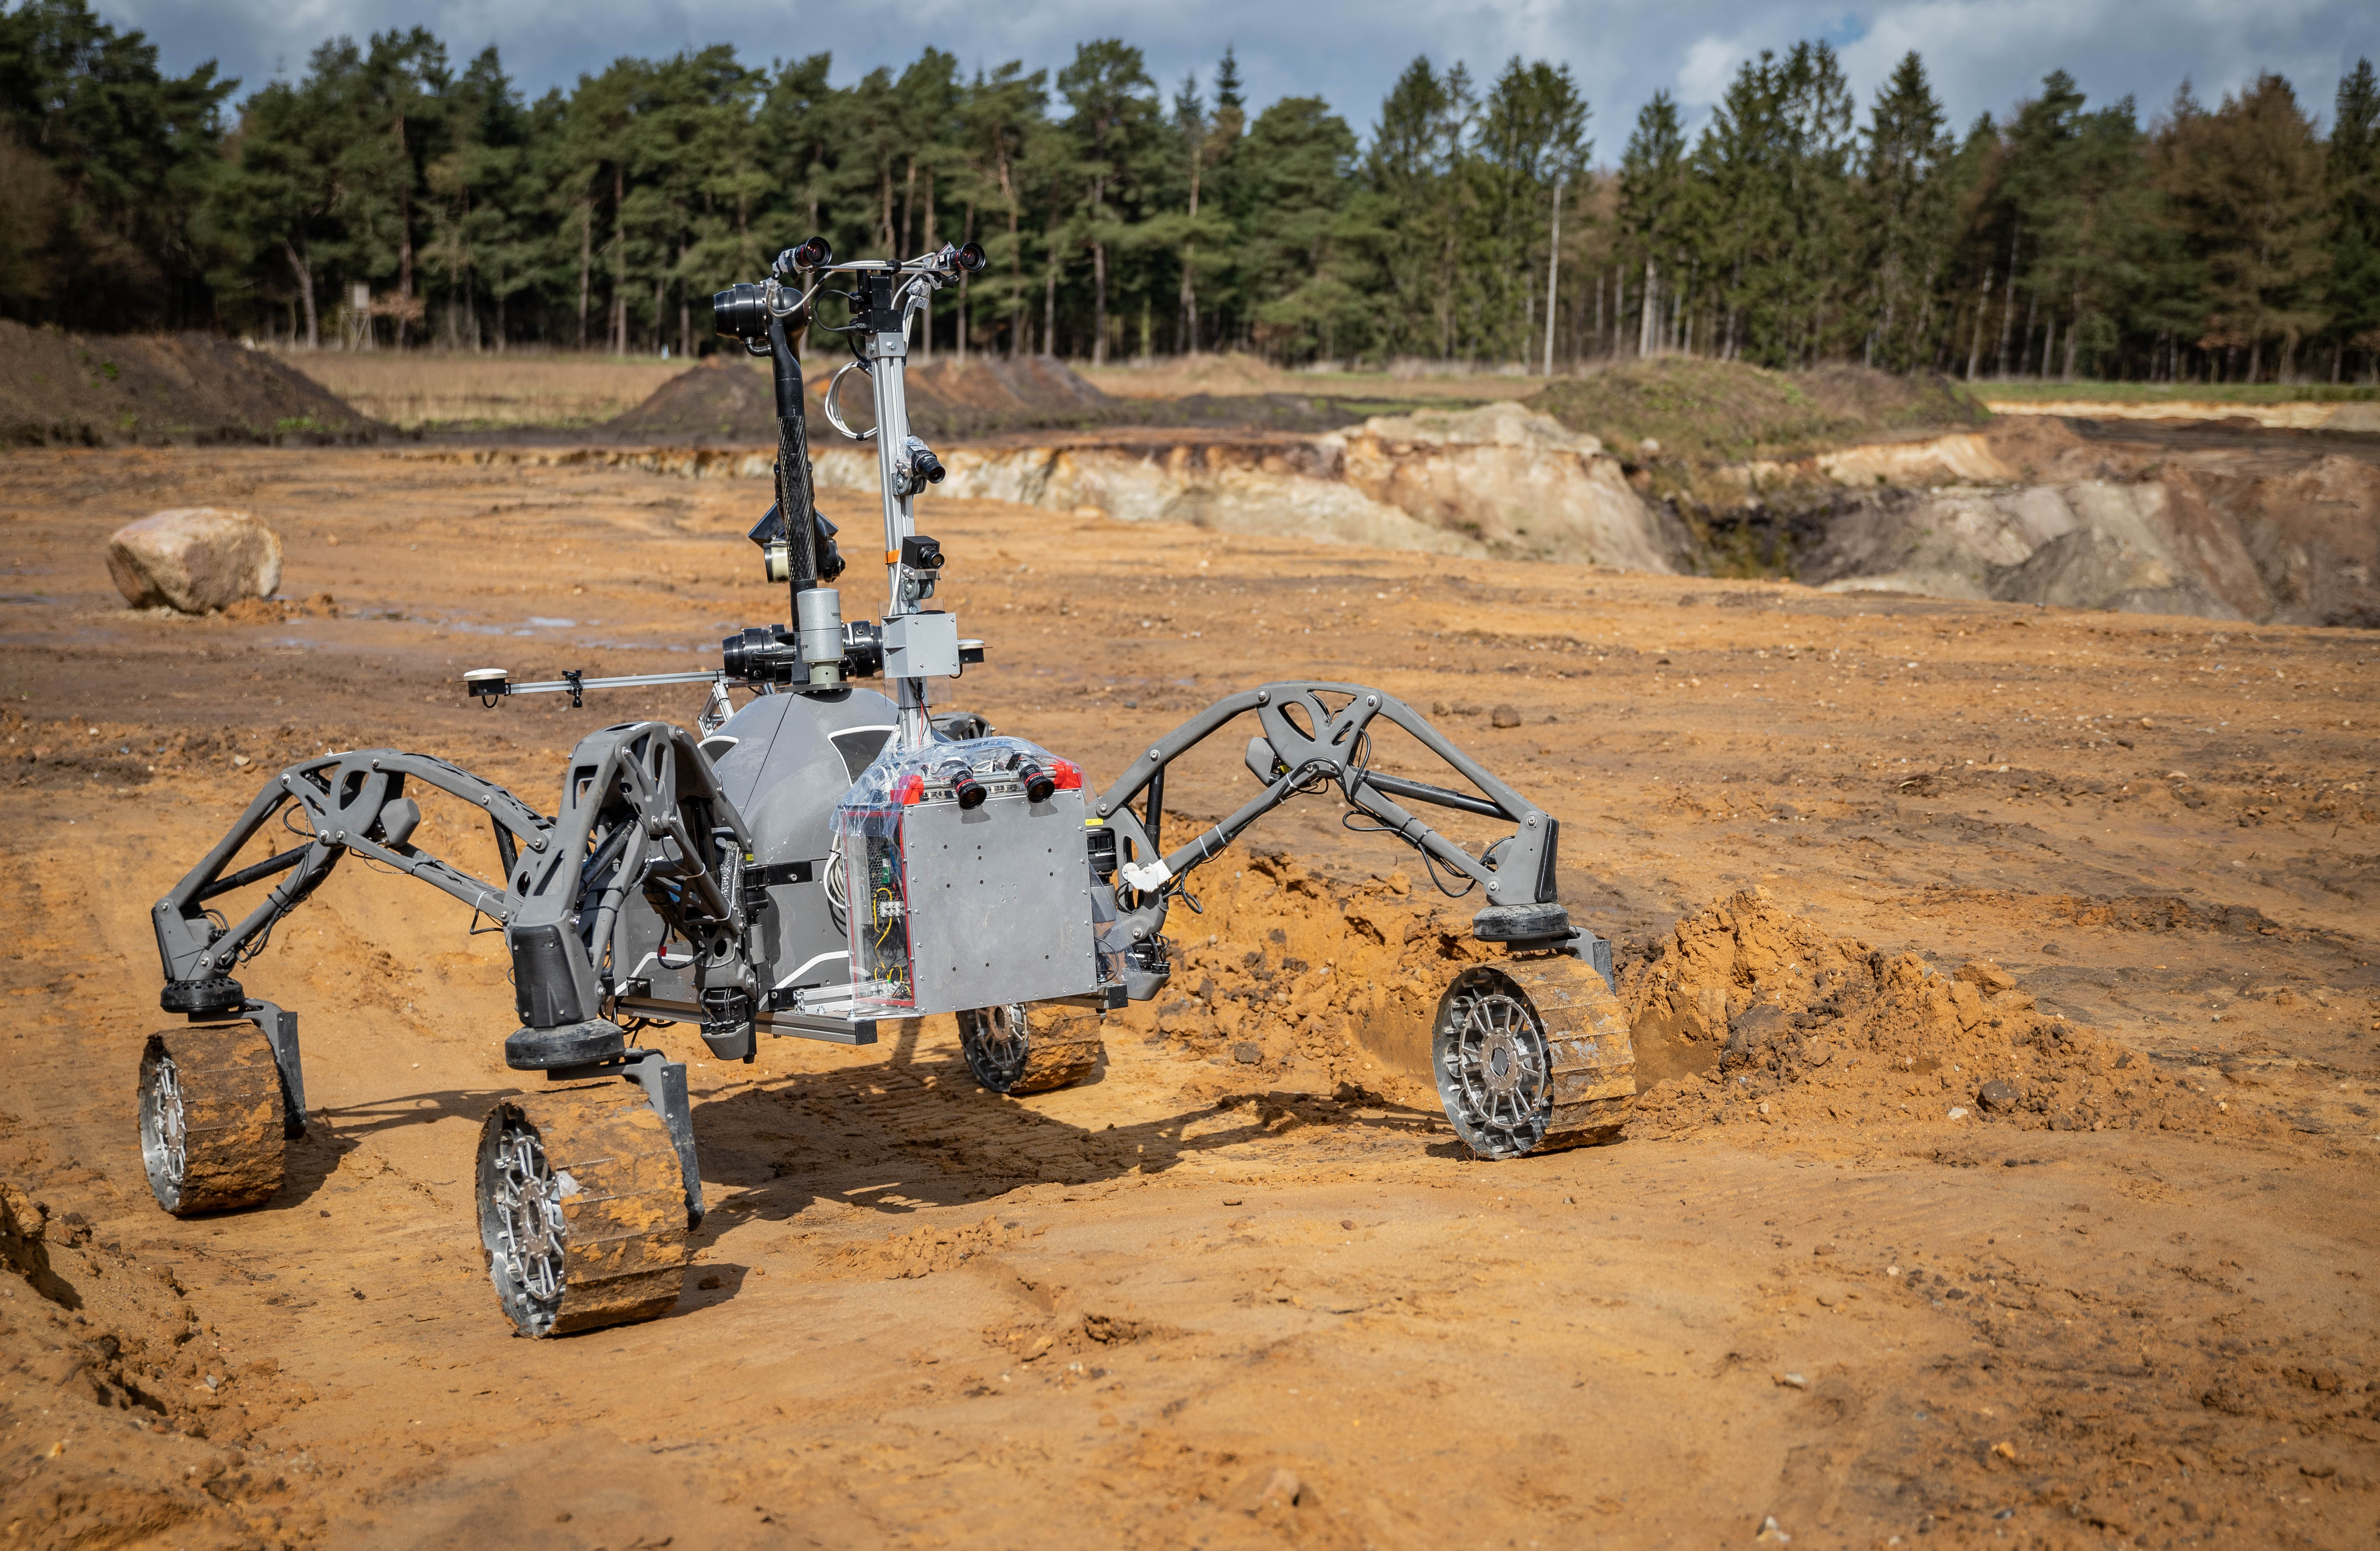
\includegraphics[width=0.4\textwidth]{../figures/sandmine_v2.jpg}
    \caption{The analog site where the classifier was tested.}
    \label{fig:finaltest}
\end{figure}


\subsection{Computational Performance}

%The C++ calculations and terrain classifications were executed in sufficient time in parallel to the rest of SherpaTT's Motion Control System, on a single thread, using a i7 processor with a CPU clock speed of 4.6 GHz.
The execution time of the code has been repeatedly measured. 
Since the computation is executed on a single thread, the execution time can be identified measuring the averaged wall time of the code execution. 
The resulting execution time depends on the threading of the operating system which is in this case is the Linux distribution Ubuntu 18.04 LTS, the same that the onboard system of SherpaTT used during the experiments. 
The time measures have been taken on an i7 processor with a CPU clock speed of 4.6 GHz. 
Table~\ref{table:compmeasurments} shows the results of these measurements. 

%\clearpage

\begin{table}[htb!]
   \centering
    \begin{tabularx}{\columnwidth}{X|XXX}
        \textbf{Method:} & \multicolumn{3}{X}{Wall Time [$ms$]} \\
        &min.&max.&avg.\\
        \hline
        \hline
        \textbf{calculateFeatures():} & 9&  17.1& 13.2 \\
        \textbf{calculateStat():}     & 6.3 & 13 & 7.1 \\
        \textbf{svmPredict():}        &  0. &  0.001 & 0.0007  \\
        \hline
        \textbf{overall:}             & 15.3 & 30.1 &20.3  \\
    \end{tabularx}	
    \caption{Wall time measurements of the methods of the C++ classification library.}
    \label{table:compmeasurments}
\end{table}

As the averaged execution time of the C++ classification library is 20.3 $ms$ this could lead to the delay of the next data collection step which are done every 10 $ms$ and hence cause the drop of one data sample per second. 
The drop of one data sample of the one hundred data samples that are strapped every second is assumed to be acceptable.


\section{Conclusions}

The presented work explains the implementation of a terrain classifier, which has been deployed and tested onboard of the hybrid locomotion robotic platform SherpaTT.
It has been shown that the SVM classifier provides useful results and can be run onboard along the rest of the software components.

The classification results on the test data collected along with the training data yield a 93\% of overall accuracy. 
These results have been improved using Deep Learning techniques as shown in \cite{ugenti2021}. 
Thus, in the near future we aim to integrate and test this approach onboard of the system.
During field tests a new type of surface was encountered that did not corresponded to any known class by the classifier. 
Nevertheless the two closest surface types were selected, which we interpret as a robust response.
In the future, this could be improved by combining the approach with an unsupervised technique to automatically identify anomalies and potentially generate new types of surfaces.

% Outlook applications
The applications of the terrain classifier will include contributions to the environment modelling while traversing and the use of the terrain class to adapt various navigation settings.
Besides the final class of terrain, the module computes physical properties of the surface and yields valuable environmental information. 
These features can be used in future missions to predict errors in the localization, e.g. due to different friction coefficients or to generate more realistic contact simulations to further improve the control of the system.
The terrain type has to be taken into account, when setting the costs for the potential paths traversing the corresponding regions. 
For instance, paths over a slope of certain inclination may be traversed if the surface is composed of a material with high friction, but the same task could become very challenging if the friction coefficient on that surface is low. 

\clearpage
%\FloatBarrier

\bibliographystyle{alpha}
\bibliography{sherpatt_terrain_classifier.bib}

\end{document}
